% article draft @ https://www.overleaf.com/11039646jmkfnhxvqpfp
\documentclass[oneside,12pt]{article}
\usepackage[a5paper,margin=5mm]{geometry}%,showframe
%\usepackage{showframe}
\usepackage[utf8]{inputenc}
\usepackage{xcolor}
\usepackage[colorlinks,
	linkcolor={red!50!black},citecolor={blue!50!black},urlcolor={blue!80!black}]{hyperref}

%% cross references [hrefs]
\usepackage{caption}
\def\figureautorefname~#1\null{fig.#1}
\newcommand{\email}[1]{$<$\href{#1}{#1}$>$}

%% figures
\usepackage[pdftex]{graphicx}
\newcommand{\fig}[4]{
\begin{figure}[h]
{\centering\noindent\includegraphics[#4]{#1}
\protect\caption{#3}\label{fig:#2}}
\end{figure}
}
\newcommand{\figref}[1]{$[$fig.{\ref{#1}}$]$}

% relative sectioning
\usepackage{ifthen}
\newcounter{secdepth}\setcounter{secdepth}{0}
\newcommand{\secup}{\addtocounter{secdepth}{1}}
\newcommand{\secdown}{\addtocounter{secdepth}{-1}}
\newcommand{\secrel}[1]{
\ifthenelse{\equal{\value{secdepth}}{0}}{\part{#1}}{}
\ifthenelse{\equal{\value{secdepth}}{-1}}{\chapter{#1}}{}
\ifthenelse{\equal{\value{secdepth}}{-2}}{\section{#1}}{}
\ifthenelse{\equal{\value{secdepth}}{-3}}{\subsection{#1}}{}
\ifthenelse{\value{secdepth} < -3}{\subsubsection{#1}}{}
}
\newcommand{\secly}[1]{\section*{#1}\addcontentsline{toc}{section}{#1}}
\newcommand{\subsecly}[1]{\section*{#1}\addcontentsline{toc}{subsection}{#1}}

% misc

\renewcommand{\emph}[1]{\textbf{#1}}

% [nosep] option in lists/enums
\usepackage{enumitem}
% frame box
\usepackage{framed}

%% languages/programs

\newcommand{\prog}[1]{\textit{#1}}
\newcommand{\lang}[1]{$#1$}

\newcommand{\C}[1]{\lang{C_{#1}}}
\newcommand{\cpp}{\lang{C_{+^+}}}

\newcommand{\prolog}{\lang{Prolog}}
\newcommand{\xsb}{\prog{XSB}}

\newcommand{\neo}{\prog{neo4j}}



\title{
Using active hypergraph database\\
as software development approach:\\
\Huge{Graph Driven Programming}}

\author{\small{\copyright\ Dmitry Ponyatov \email{dponyatov@gmail.com}, free researcher, 2017}}

\begin{document}
\maketitle
\begin{abstract}\noindent
Software development and program architecture engineering has grows complexity
in last decades. The existing zoo of programming languages, para\-digms,
hardware platforms and operating systems, combined with the software development
market requirements, exceeds the capabilities of a particular individual
developer. Thus, it is required to create a powerful tool for compensation of
software systems development complexity, that combines design tools, RAD, MDP,
simulation debugging, static and dynamic analysis of programs, parallel
computing support, and, first of all, \emph{an expert system and knowledge bases
provides knowledge storage, fuzzy search and inference} not only in software
engineering, but also in applied fields (mathematics and numerical methods,
physics, chemistry, mechanics and structural engineering, CAD, electronics,
digital signal processing, business planning, accounting and logistics, task and
time management, etc).
\end{abstract}

\tableofcontents\secdown\secdown

\secly{Introduction}

Software development and program architecture engineering has grows complexity
in last decades. This problem is especially notable in hard real-time control
systems applied in safety-critical domains: avionics, aerospace, automobiles,
and medicine, and covered by tons of safety reglaments and standards.
\cite{book1}

If we look on some random typical software developer vacancies, we see huge
amount of conventional requirements on knowledge and skills (emphasized in
text), making developer live damn scary: to make yourself promising in your
profession, you must spend an everyday self-learning in your work and spare
time.

\begin{framed}\noindent
An experienced \emph{Java} programmer with \emph{R} experience is sought to
participate in the continued design and development of a flexible, open-ended
platform for \emph{bioinformatics} data integration, \emph{analysis}, and
\emph{visualization}. This open-source platform \emph{distributes computations}
across client, server, and \emph{grid} components. The candidate is expected to
contribute to architecture design, \emph{visualization}, and \emph{web-GUI}
implementation, \emph{integration} of \emph{existing algorithms}/programs,
troubleshooting software bugs, and producing technical documentation. The
position requires a Bachelor's Degree in \emph{Computer Science},
\emph{Engineering}, \emph{Mathematics}, \emph{Physics}, \emph{Bioinformatics},
or in a similar field or equivalent in education and experience, plus a minimum
of three (3) years of related experience. At least 1 year of experience
\emph{programming in a UNIX environment} is required, as well as 1 year of
experience with \emph{R} and \emph{Java} programming, including experience with
distributed file systems and cluster compute management, shell scripting on UNIX
and experience in one scripting language, preferably \emph{Python}. Also
desirable is familiarity with \emph{database} driven projects using \emph{MySQL}
or a similar database system, \emph{SQL}, \emph{JDBC}, \emph{Linux}, and use of
appropriate IDEs (e.g., \emph{Eclipse}), project management tools (e.g.,
\emph{ant}, \emph{subversion}), web technologies (web service frontend triple
\emph{HTML}/\emph{CSS}/\emph{JavaScript}, \emph{tomcat}, \emph{php},
\emph{drupal}).
\end{framed}

\begin{framed}\noindent
Participate on requirement analysis, design, development and \emph{testing}.\\
Knowledge developing and debugging using \emph{C} (Kernel)/\emph{C++}, \emph{BASH} \\
Expert knowledge with \emph{algorithm and data structure} design \\
Strong knowledge and extensive \emph{Python}/\emph{UNIX}/Linux development skills \\
Knowledge of programming for computer networking IP protocol set, \emph{TCP/IP}, branch to interoffice connectivity, \emph{network security}, and \emph{encryption} is a must \\
Related Terms: C (\emph{Linux kernel development}), \emph{C++}, \emph{Python}, \emph{Perl}, Linux, UNIX, BASH, \emph{XML}, \emph{TCP/IP} and \emph{SSL}\\
Participate on requirement analysis, design and development on \emph{Java}, \emph{J2EE}, \emph{C/C++}. Develop applications, work on \emph{Amazon Web Services}, work on integrated development environments. Requires B.S. degree in Computer Science or related area plus 5 years of experience in software development, or, alternatively, M.S. degree in Computer Science or related area. Knowledge of Java, J2EE, C/C++, \emph{JSF}, \emph{Servlets}, \emph{JSP}, \emph{Java Web Services}, \emph{XML}, \emph{Ajax}, \emph{jQuery}, \emph{HTML} and \emph{CSS}; familiarity with technologies like \emph{JDBC}, \emph{SOAP} and \emph{OOD}; knowledge of \emph{PL/SQL} Procedures, Functions and Triggers for \emph{Oracle}, \emph{MySQL} and \emph{SQL Server} databases; ability to work on \emph{Linux Kernel} module, \emph{TCP/IP stack} application and \emph{network protocols} implementation; familiarity with \emph{XML} documents and use of \emph{DTD}, \emph{SCHEMA} and parsing using \emph{SAX}, \emph{DOM} and transformations using \emph{XSL}, \emph{XSLT}, and \emph{XPATH}.
\end{framed}

\begin{framed}\noindent
\begin{itemize}[nosep,leftmargin=*]
\item Design, develop, and release sophisticated Windows GUI applications in an iterative environment using \emph{C\#} \emph{.NET}, \emph{Windows Forms}, and the \emph{Win32 API}
\item At least 2 years Windows GUI programming (C\# .NET, Windows Forms, \emph{WPF}, Win32 API)
\item \emph{JavaScript} single page application development (AngularJS, Knockout.JS or similar)
\item Familiarity with \emph{SQL} and \emph{databases}
\item Experience with DevExpress Windows Forms/WPF  UI Framework
\item Experience with \emph{financial software} and/or financial trading, especially in fixed income, a plus
\item Experience with \emph{real-time systems} and rapid iterations a plus
\item Experience with \emph{Multithreading} and Interfacing with \emph{TIBCO}
\item Knowledge of \emph{VB}, \emph{Python}, \emph{C++}
\item Experience with \emph{Subversion} Source Control
\item Experience with \emph{Unit Testing}, Automated UI Testing, and Code Coverage tools.
\item Knowledge of S.O.L.I.D principles, Requirement Analysis, and QA Test Management
\item Experience using tools like ReSharper, Beyond Compare,  Tortoise
\end{itemize}
\end{framed}

\begin{framed}\noindent
\begin{itemize}[nosep,leftmargin=*]
\item \emph{C programming} experience
\item Software Development using '\emph{Internet of Things}' standards, including \emph{OCF}
\item Software Development using IP based \emph{internet protocols} including \emph{SSDP}, \emph{UDP}, \emph{TCP}, \emph{TLS}, CoAP, \emph{HTTP}, \emph{MQTT}, Thread, \emph{WiFi}, WebSockets
\item Development on \emph{Windows} (\emph{Win32 API}, \emph{.NET}) and Linux/\emph{Unix} Platforms
\item Managing microservices in \emph{AWS}
\item \emph{Testing} and debugging \emph{embedded electronics}
\item Rapid prototyping using available tools such as: \emph{Arduino}, \emph{Raspberry} Pi
\item Experience and continued interest in learning and \emph{deploying} unfamiliar languages, \emph{frameworks}, and other tools
\item \emph{Python} or \emph{Shell} Scripting language familiarity
\item Eager to learn and adapt to new and \emph{changing requirements}
\item Bachelor's degree in ECE, EE, CS or related field.
\item \emph{AWS} experience or other \emph{cloud providers}
\end{itemize}
\end{framed}

My previous job was linked with hardware and firmware design. So my thoughts was
about it will be great to have some Wolfram Alpha like expert system with lot of
engineering knowledge databases (basic three sciences Math/Physics/Chemistry,
Electronics, Computer Science and Programming, especially software synthesis
using Model Driven programming, Digital Methods and DSP), which can help me in
my work.

First I dig into pure Prolog and read lot of books on expert systems design, and
in result it was no progress at all. In my first senses, Prolog is only able to
implement knowledge bases about siblings.

So in last year I faced with graph databases, especially neo4j, and it looks
great for knowledge representation, and processing via graph rewrite. I feel
that graphs can be natively represented in form of Prolog (especially
\href{https://en.wikipedia.org/wiki/HiLog}{HiLog}) clauses (edge as predicate,
and nodes as arguments), so for inference purposes it looks able to export graph
into some modern Prolog system like
\href{http://flora.sourceforge.net/}{Ergo/Flora} or XSB, do inference, and push
back results via graph rewrite requests. Or inference can be done at graphdb
engine level using some custom plugin.

\secrel{Graph Data Model}\secdown

For first time we will use attribute graph model. Nodes represents data
elements, and edges or links shows relationships between nodes. Nodes and edges
can have properties. \neo\ also includes special case of properties\ --- labels,
you can think about label as property without value, or has value equal to
itself.

So graph structure can represent wide range of different things, look at your
whiteboard with some schemes for example. Let’s look on our prototype system
architecture at \autoref{fig:architecture}. As you can see that there is no
reason to add any extra notes: all knowledge embodied in this graph is visually
understandable. As other example, see \autoref{fig:mobile} later.

\fig{fig/architecture.png}{architecture}{Active graph system
architecture}{width=\textwidth}

\clearpage

\secrel{Graph Databases}\secdown

Most graph databases uses data models, not so powerful to implement graphs shown
on figures \autoref{fig:architecture},\autoref{fig:mobile} natively. As you can
see, there is some elements not supported: grouping and containers, links on
links, N-ary relations with \mbox{$N>2$} (and custom visualization
representations). Some of this can be described in hypergraph (see
\autoref{hyper}), but for currently existing graphdb engines we need some
transformations.

\secrel{\neo}

The most simple and easy install graph database is
\href{https://neo4j.com/}{\neo}. It has lot of data model limitations, in detail
described in \autoref{hyper}\ section, but we will use \neo\ as graph storage
for our prototype system, ready to use just now:

\begin{itemize}[leftmargin=*]
  
\item
install
\href{http://www.oracle.com/technetwork/java/javase/downloads/index.html}{\java\
SE} for your system\note{install full
\href{http://www.oracle.com/technetwork/java/javase/downloads/jdk8-downloads-2133151.html}{JDK}
if you not limited in disk space, or 
\href{http://www.oracle.com/technetwork/java/javase/downloads/jre8-downloads-2133155.html}{JRE}
only}.
Download .tag.gz package and
unpack it in user home directory, or somewhere else
\begin{verbatim}
user@unix$ cd ~ ; tar zx < Downloads/
\end{verbatim}

\item
add to \verb|JAVA_HOME| and \verb|PATH| environment variables points to your
\java\ install/bin directory

add to file \verb|~/.profile|
\begin{verbatim}
. ~/.setenv
\end{verbatim}
add file \verb|~/.xsessionrc|
\begin{verbatim}
. ~/.setenv
\end{verbatim}
add file \verb|~/.setenv|
\begin{verbatim}
export JAVA_HOME="/home/user/jdk1.8.0_131"
export PATH="$JAVA_HOME/bin:$PATH"
\end{verbatim}

\item
download \href{https://neo4j.com/download/community-edition/}{\neo\ community
edition} distribution archive and unpack it by commands:
\begin{verbatim}
unix:~$ tar zx < Downloads/neo4j-community-3.2.3-unix.tar.gz
\end{verbatim}
\begin{verbatim}
windows> unzip Downloads/neo4j-community-3.2.3-windows.zip
\end{verbatim}

\item 

start \neo\ server in console mode (recommended) from your home directory:
\begin{verbatim}
user@unix$ ~/neo4j-community-3.2.3/bin/neo4j console
\end{verbatim}
or in daemon mode under current user
\begin{verbatim}
user@unix$ ~/neo4j-community-3.2.3/bin/neo4j start
\end{verbatim}
You can stop \neo\ server by pressing \keys{Ctrl-C}\ in console or run stop
command in daemon mode
\begin{verbatim}
user@unix$ ~/neo4j-community-3.2.3/bin/neo4j stop
\end{verbatim}
If your Java was not installed properly, you will get errors like
\begin{verbatim}
ERROR: JAVA_HOME is incorrectly defined
as /home/ponyatov/jdk1.8.0_131
\end{verbatim}
(the executable \verb|/home/ponyatov/jdk1.8.0_131/bin/java| does not exist)

Also you can install only JRE and run \neo\ with directly selected Java runtime
directory:
\begin{verbatim}
user@unix$ JAVA_HOME=~/jre1.8.0_144 \
    ~/neo4j-community-3.2.3/bin/neo4j console
\end{verbatim}

\item connect to \url{http://localhost:7474/}\ with any JavaScript-enabled web
browser

\item connect to graphdb server via command
\begin{verbatim}
:server connect
host: bolt://localhost:7687
username: neo4j
password (default): neo4j
\end{verbatim}
\menu{Connect}

\item you will be asked for new password for \neo\ user
\begin{verbatim}
New password: ********
Repeat new password: ********
\end{verbatim}
\menu{Change password}
  
\end{itemize}
\secup

\secrel{Sample program graph model}

For demo purposes let’s see simple program for UNIX in pure \C{}:

\lst{src/hello.c}{hello.c}{Hello World}

\fig{fig/hello.png}{hello}{Hello World simple program
in \C{}}{width=\textwidth}

Here we see types taxonomy for primitive subset of \C{}\ language, \verb|main()|
function with arguments and \verb|return| statement. Note that function
arguments in \C\ must be ordered, so we use \emph{next} relation to add this
order. Other notable thing is double return relation of main() function: this is
sample of inherited relation\ --- \verb|(main:function)-[:return]->(int:type)|
relation was inherited from first \verb|main-[:return]->(0:int)| relation
corresponds to \verb|return 0| statement. \textbf{ako} (a-kind-of, superclass)
and \textbf{isa} (is-a) relations corresponds to inheritance and instantiation.


\secup


\noindent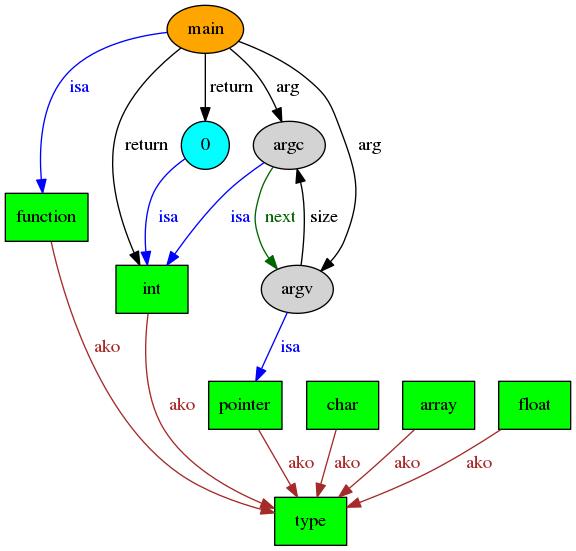
\includegraphics[width=\textwidth]{fig/hello.png}

\noindent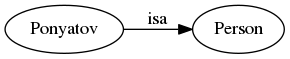
\includegraphics[width=0.5\textwidth]{fig/person.png}

\addcontentsline{toc}{section}{List of Figures}
\listoffigures

\begin{thebibliography}{99}
\addcontentsline{toc}{section}{References}

\bibitem{book1}
\href{https://insights.sei.cmu.edu/sei_blog/2015/09/managing-software-complexity-in-models.html}{\textbf{Managing
Software Complexity in Models}}\\

\bibitem{book2}
\href{https://www.repository.cam.ac.uk/bitstream/handle/1810/247929/Urma%20and%20Mycroft%202013%20Science%20of%20Computer%20Programming.pdf}{\textbf{Source-Code
Queries with Graph Databases\ --- with Application to Programming Language Usage and Evolution}}\\
\textit{Raoul-Gabriel Urma, Alan Mycroft}\\
Computer Laboratory, University of Cambridge

\bibitem{book3}
\href{http://www3.cs.stonybrook.edu/~kifer/TechReports/flogic.pdf}{\textbf{Logical
Foundations of Object-Oriented and Frame-Based Languages}}\\
\textit{Michael Kifer, Georg Lausen, James Wu}

\bibitem{minsky}
\href{https://web.media.mit.edu/~minsky/papers/Frames/frames.html}{\textbf{A
Framework for Representing Knowledge}}\\
\textit{Marvin Minsky}\\
MIT-AI Laboratory Memo 306, June, 1974.

\bibitem{bluebook} 
\href{http://stephane.ducasse.free.fr/FreeBooks/BlueBook/Bluebook.pdf}{\textbf{Smalltalk-80:
The Language and its Implementation}}\\
\textit{Adele Goldberg , DavidRobson}\\
Xerox Palo Alto Research Center\\
Addison Wesley, 1983.\\
ISBN 0-201-11371-6.\\

\bibitem{Rodriguez}
\href{https://markorodriguez.com/2011/02/23/knowledge-representation-and-reasoning-with-graph-databases/}{Knowledge
Representation and Reasoning with Graph Databases}\\
\textit{Marko A. Rodriguez}

\end{thebibliography}

\end{document}
